The memory efficient attention refers to this paper\cite{DBLP:journals/corr/abs-2112-05682}.
The LSE trick refers to this blog\cite{lse-trick}.

\subsection{\href{https://github.com/HazyResearch/flash-attention/blob/main/flash_attn/flash_attn_triton.py}{The triton implementation}}

Softmax function is computed as follows:

\begin{align*}
    \text{softmax} &= \frac{\text{exp}\left(x_i -c\right)}{\sum_{i}\text{exp}\left(x_i -c\right)} \\
    &c = \text{max}(x_1,\ldots, x_n)
\end{align*}

The LogSumExp(LSE) is a smooth maximum.

\begin{align*}
    \text{LSE}(x_1, \ldots ,x_n) &= \text{log}\left( \text{exp}\left(x_1\right)+\cdots+\text{exp}\left(x_n\right)\right) \\
    &=c + \text{log}\sum_{n}\text{exp}(x_i - c) \\
    &c = \text{max}(x_1,\ldots, x_n)
\end{align*}

$lse_i$, $m_i$ and $acc\_o$ are accumulators.

$lse_i=\textbf{\textit{-inf}}$

$m_i=\textbf{\textit{-inf}}$: maximum up to the previous block.
$m_{ij}$ maximum up to the current block.

$acc\_o = \vec{\textbf{\textit{0}}}$.


\begin{align}
    &\textbf{\textit{Iterate }} (k,v)\ \text{in} \ K,V\ : \nonumber\\
    &\qquad qk = \text{dot}(q,k) \\
    &\qquad m_{ij} = \text{max}(\text{max}(qk), lse_i) \label{eq:2}\\
    &\qquad p = \text{exp}(qk-m_{ij}) \\
    &\qquad l_{ij} = \text{sum}(p) \\
    &\qquad \textcolor{grey}{\textit{// renormalize o}} \nonumber\\
    &\qquad acc\_o\_scale = \text{exp}(m_i - m_{ij}) \\
    &\qquad acc\_o = acc\_o\_scale * acc\_o \\
    &\qquad acc\_o = acc\_o+\text{dot}(p, v)  \\
    &\qquad \textcolor{grey}{\textit{// update statistics}} \nonumber\\
    &\qquad m_{i} = m_{ij} \\
    &\qquad l_{{i}\_{new}} = \text{exp}\left( lse_i - m_{ij}\right) + l_{ij} \label{eq:9}\\
    &\qquad lse_{i} = m_{ij} + \text{log}(l_{i\_new}) \\
    &\textcolor{grey}{\textit{// o\_scale is the denominator of the softmax function}} \nonumber\\
    & o\_scale = \text{exp}(m_i - lse_i) \label{eq:11}\\
    &acc\_o = acc\_o * o\_scale
\end{align}

In \cref{eq:2} $lse_i$ is used as the approximation of max.

The first component of the right hand side of \cref{eq:9}:

\begin{align*}
    \text{exp}\left( lse_i - m_{ij} \right)&= \text{exp}\left(c_{old} + \text{log}\sum_{n}\text{exp}(x_i - c_{old}) - c_{new}\right) +l_{ij}\\
    &= \text{exp} \left( \left(c_{old}-c_{new}\right) + \text{log}\sum_{n}\text{exp}(x_i - c_{old}) \right) \\
    &= \text{exp}\left( c_{old} - c_{new}\right)\sum_{n}\text{exp}(x_i - c_{old})\\
\end{align*}

$o\_scale$ in equation \cref{eq:11} is the denominator of the softmax function.
\begin{align*}
m_i - lse_i&= \text{exp} \left(c - c - \text{log}\sum_{n}\text{exp}(x_i - c)\right) \\
&= \text{exp} \left(- \text{log}\sum_{n}\text{exp}(x_i - c)\right)\\
&= \text{exp} \left(\text{log}\frac{1}{\sum_{n}\text{exp}(x_i - c)}\right)\\
&=\frac{1}{\sum_{n}\text{exp}(x_i - c)}
\end{align*}

\newpage
\subsection{How was Flash Attention's Formula Derived}

\begin{equation}
\text{Attention}(Q, K, V)=\text{softmax}(QK^T)V \label{attn:softmax}
\end{equation}
where $Q, K, V\in \mathbb{R}^{N\times d}$ are sequences of vectors.

We expect that \textcolor{byzantium}{the \textbf{entire} computational process of equation (\ref{attn:softmax}) can proceed block by block, with each block computing a portion of the final result}.
If the block size is chosen appropriately, the entire computational process can be kept in high-speed memory.
We expect the computational process to proceed as follows:
\lstset{
  frame=lrtb,
  backgroundcolor=\color{aliceblue},
  numbers=left,
  numbersep=1em,
  xleftmargin=1em,
  breaklines=true,
  linewidth=\linewidth
}
\begin{lstlisting}[language=code_example2, caption={}]
// stage1: local reducer computes partial results on individual blocks
(:$o_1$:) = Attention((:$q, ks_1, vs_1$:))     (:$o_2$:) = Attention((:$q, ks_2, vs_2$:))

// stage2: combine partial results
(:$o_{\text{new}}=\text{Combiner}(o_1,o_2)$:)
\end{lstlisting}
\textcolor{byzantium}{During the first stage, each local reducer computes a partial result on an individual block; during the second stage, these partial results are combined to obtain the correct final result}.
Thus, the problems are:
\begin{enumerate}
\item Under what conditions can the entire computational process be decomposed into these two stages, and is there a combiner that can compute the correct final result?
\item If such a combiner exists, how can it be constructed
\end{enumerate}

Let's see how was Flash Attention's formula derived.

$q\in \mathbb{R}^d$ is a vector (the smallest block of $Q$). $ks_1, ks_2, vs_1, vs_2 \in \mathbb{R}^{B \times d}$ are sequences of vectors. They are blocks of $K$ and $V$. $B$ are block size.

\begin{align*}
  &a_1 = \text{dot}(q, ks_1) &a_2 &= \text{dot}(q, ks_2) \\
  &b_1 = \textcolor{red}{\max}(-\inf, a_1) &b_2 &= \textcolor{red}{\max}(-\inf, a_2) \\
  &c_1 = a_1 - b_1 &c_2&= a_2 - b_2 \\
  &d_1 = \exp(c_1) &d_2&=\exp(c_2) \\
  &e_1 = \textcolor{red}{\text{sum}}(0, d_1)&e_2&=\textcolor{red}{\text{sum}}(0,d_2) \\
  &f_1 = \frac{d_1}{e_1}&f_2&=\frac{d_1}{e_1} \\
  &g_1 = f_1 *vs_1 &g_2&=f_2 * vs_2 \\
  &o_1 = \textcolor{red}{\text{sum}}(0, g_1) &o_2 &= \textcolor{red}{\text{sum}}(0, g_2) \\
\end{align*}

$b = \max(b_1, b_2)$, $\triangle c_1 := b_1 - b$ $\triangle c_2 := b_2 - b$

$
\begin{bmatrix}
  a \\
  \textcolor{red}{b} \\
  c \\
  d \\
  \textcolor{red}{e} \\
  f \\
  g \\
  \textcolor{red}{o}
\end{bmatrix} = 
\begin{bmatrix}
  a_1 \\
  \textcolor{red}{b_1} \\
  c_1 \\
  d_1 \\
  \textcolor{red}{e_1} \\
  f_1 \\
  g_1 \\
  \textcolor{red}{o_1}
\end{bmatrix} \bigoplus
\begin{bmatrix}
a_2 \\
\textcolor{red}{b_2} \\
c_2 \\
d_2 \\
\textcolor{red}{e_2} \\
f_2 \\
g_2 \\
\textcolor{red}{o_2}
\end{bmatrix} = 
\begin{bmatrix}
[a_1:a_2] \\
\textcolor{red}{\max(b_1, b_2)} \\
\left[c_1 + \triangle c_1 : c_2 +\triangle c_2\right] \\
\left[d_1 \exp(\triangle c_1):d_2 \exp (\triangle c_1)\right] \\
\textcolor{red}{e_1 \exp(\triangle c_1)+ e_2 \exp(\triangle c_2)} \\
\left[\frac{\exp (c_1 + \triangle c_1)}{e_1 \exp(\triangle c_1)+ e_2 \exp(\triangle c_2)}: \frac{\exp (c_2 + \triangle c_2)}{e_1 \exp(\triangle c_1)+ e_2 \exp(\triangle c_2)} \right]\\
\left[\frac{\exp (c_1 + \triangle c_1)*vs_1}{e_1 \exp(\triangle c_1)+ e_2 \exp(\triangle c_2)}: \frac{\exp (c_2 + \triangle c_2)*vs_2}{e_1 \exp(\triangle c_1)+ e_2 \exp(\triangle c_2)} \right] \\
\frac{\exp (c_1 + \triangle c_1)*vs_1}{e_1 \exp(\triangle c_1)+ e_2 \exp(\triangle c_2)}+\frac{\exp (c_2 + \triangle c_2)*vs_2}{e_1 \exp(\triangle c_1)+ e_2 \exp(\triangle c_2)} 
\end{bmatrix}
$

\begin{align*}
  e_1'&=\text{sum}(0, d_1') \\
  &=\text{sum}(0, d_1\exp(\triangle c_1)) \\
  &=\text{sum}(0, d_1)\exp(\triangle c_1) \\
  &=e_1 \exp(\triangle c_1)
\end{align*}

\begin{align*}
o =& \frac{\exp (c_1 + \triangle c_1)*vs_1}{e_1 \exp(\triangle c_1)+ e_2 \exp(\triangle c_2)}+\frac{\exp (c_2 + \triangle c_2)*vs_2}{e_1 \exp(\triangle c_1)+ e_2 \exp(\triangle c_2)} \\
=& \frac{\exp(\triangle c_1)}{e_1 \exp(\triangle c_1)+ e_2 \exp(\triangle c_2)}\exp (c_1)*vs_1 +\frac{\exp (\triangle c_2)}{e_1 \exp(\triangle c_1)+ e_2 \exp(\triangle c_2)}\exp(c_2)*vs_2\\
\end{align*}

\begin{align*}
o_1 &= f_1 *vs_1 \\
o_1 * e_1 & = f_1 * e_1 * vs_1 \\
o_1 *e_1&=d_1 * vs_1\\
o_1 *e_1 &= \exp(c_1) * vs_1
\end{align*}

Therefore, we have:

\begin{equation}
o= \frac{\exp(\triangle c_1)}{e_1 \exp(\triangle c_1)+ e_2 \exp(\triangle c_2)}o_1*e_1 +\frac{\exp (\triangle c_2)}{e_1 \exp(\triangle c_1)+ e_2 \exp(\triangle c_2)}o_2*e_2 \label{attn:combiner}
\end{equation}

Equation (\ref{attn:combiner}) specifies how to combine the partial results of a local reducer. Suppose $b_1$, $e_1$, and $o_1$ are the outputs of another local reducer. Given a new block, the current local reducer first computes $b_2$, $o_2$, and $e_2$. The combiner then computes $b = \max(b_1, b_2)$, we set $\triangle c_1 := b_1 - b$, and $\triangle c_2 := b_2 - b$. Finally, use equation (\ref{attn:combiner}) to obtain a combined result.

\newpage
\subsection{Replace softmax with logsoftmax}

$\mathbf{x}\in\mathbb{R}^n$ is a vector.
$m(\mathbf{x}) := \max\limits_i(\mathbf{x})$

\begin{align*}
  \text{logsoftmax}(\mathbf{x}) &= \log(\text{softmax}\left( \mathbf{x} \right)) \\
  &=\log \frac{\exp\left( x_i - m\left(\mathbf{x}\right)\right)}{\sum\limits_i\exp\left( x_i-m\left(\mathbf{x}\right)\right)} \\
  &= x_i - m\left(\mathbf{x}\right) - \log \left(\sum\limits_i \exp \left( x_i -m\left(\mathbf{x}\right)\right)\right)
\end{align*}

\begin{figure}[h]
  \centering
  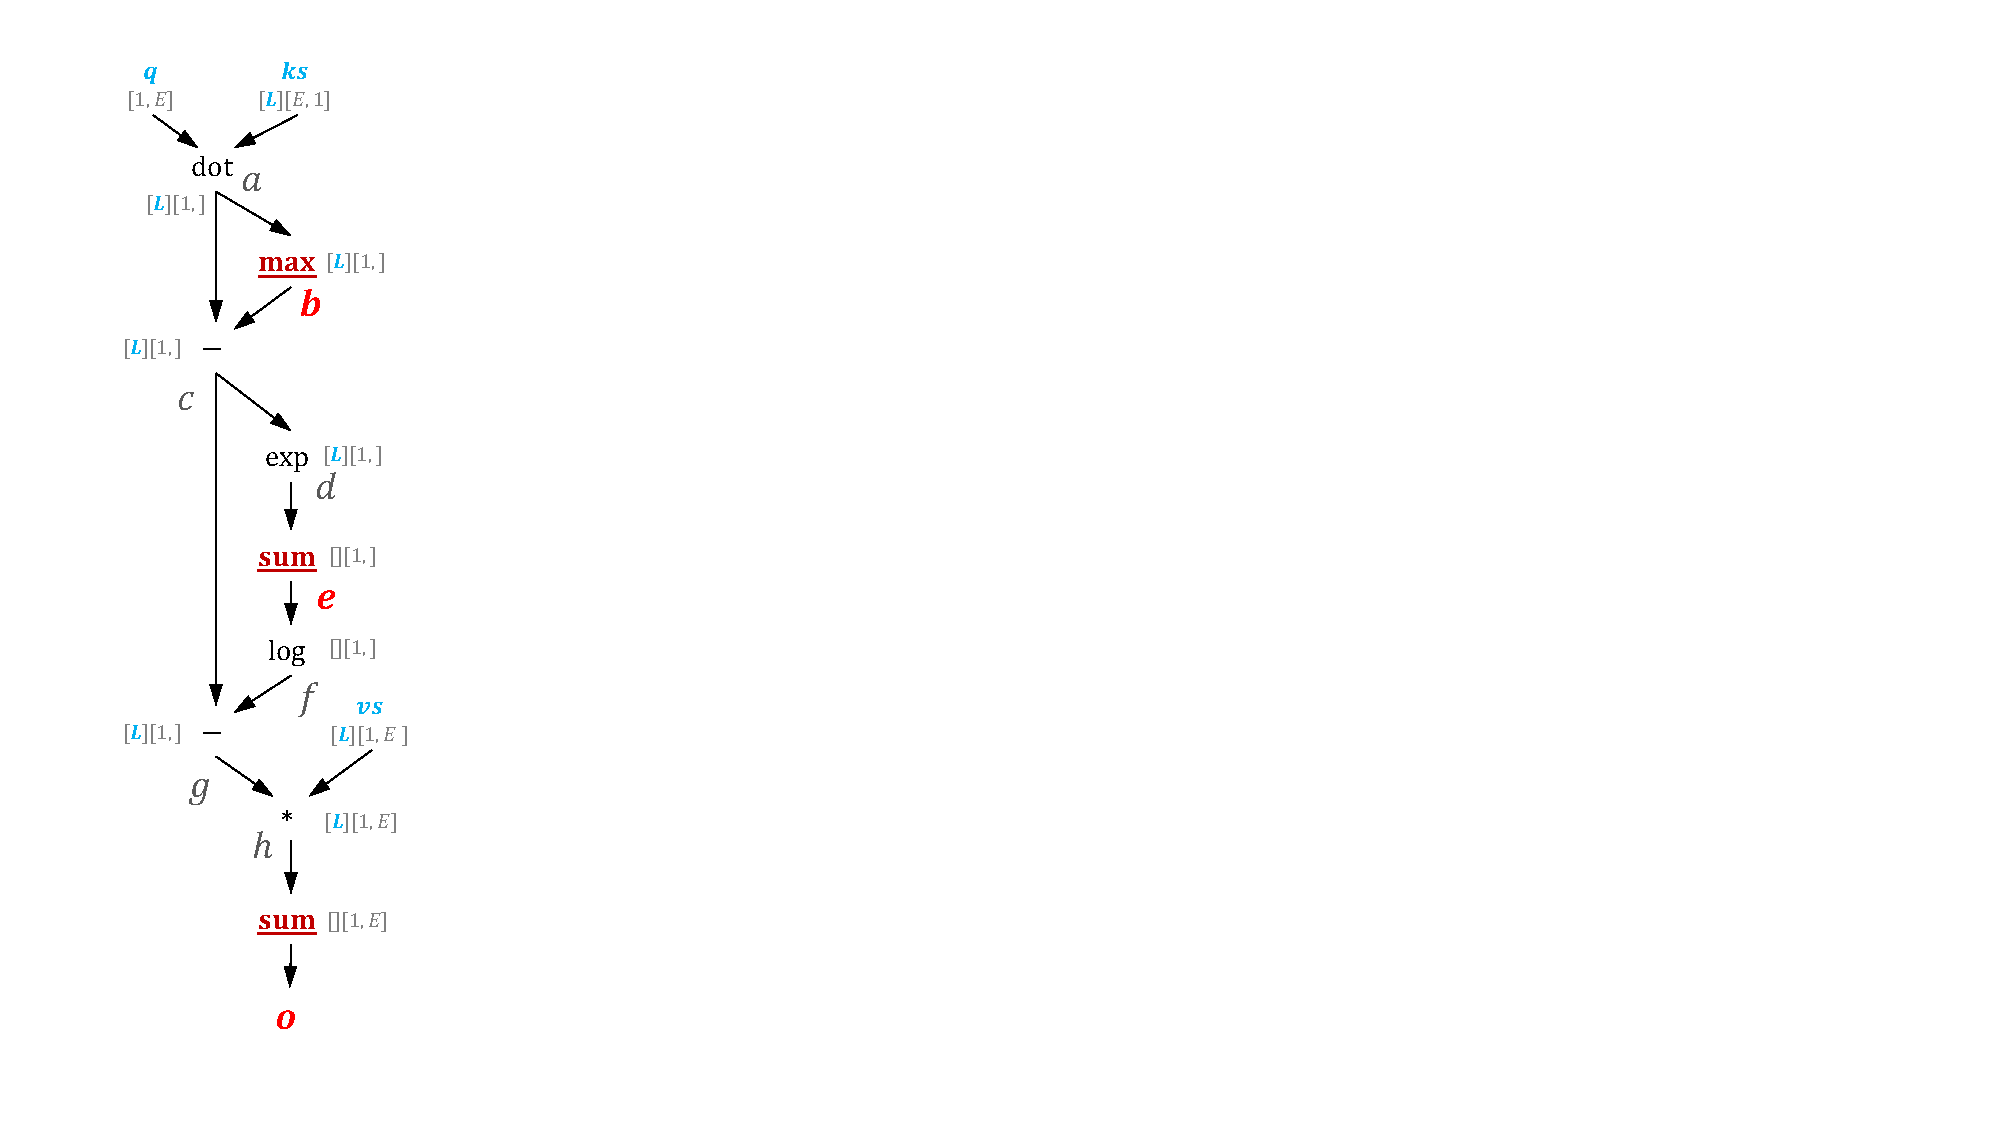
\includegraphics[width=0.2\textwidth]{figures/logsoftmax_expression_tree.pdf}
  \caption{The expression tree of logsoftmax.}
\end{figure}

\begin{align*}
&a_1 = \text{dot}(q, ks_1) &a_2 &= \text{dot}(q, ks_2) \\
&b_1 = \textcolor{red}{\max}(-\inf, a_1) &b_2 &= \textcolor{red}{\max}(-\inf, a_2) \\
&c_1 = a_1 - b_1 &c_2&= a_2 - b_2 \\
&d_1 = \exp(c_1) &d_2&=\exp(c_2) \\
&e_1 = \textcolor{red}{\text{sum}}(0, d_1)&e_2&=\textcolor{red}{\text{sum}}(0,d_2) \\
&f_1 = \log{e_1}&f_2&=\log{e_2} \\
&g_1 = c_1 - f_1 &g_2&=c_2-f_2 \\
&h_1 = g_1 * vs_1 &h_2 &= g_2 * vs_2 \\
&o_1 = \textcolor{red}{\text{sum}}(0, h_1) &o_2 &= \textcolor{red}{\text{sum}}(0, h_2) \\
\end{align*}

Equatioins in red are partial results that require a further aggregation.
Equations that consume results of these partial results requires updates.

$
\begin{bmatrix}
  a \\
  \textcolor{red}{b} \\
  c \\
  d \\
  \textcolor{red}{e} \\
  f \\
  g \\
  h \\
  \textcolor{red}{o}
\end{bmatrix} = 
\begin{bmatrix}
  a_1 \\
  \textcolor{red}{b_1} \\
  c_1 \\
  d_1 \\
  \textcolor{red}{e_1} \\
  f_1 \\
  g_1 \\
  h_1 \\
  \textcolor{red}{o_1}
\end{bmatrix} \bigoplus
\begin{bmatrix}
a_2 \\
\textcolor{red}{b_2} \\
c_2 \\
d_2 \\
\textcolor{red}{e_2} \\
f_2 \\
g_2 \\
h_2 \\
\textcolor{red}{o_2}
\end{bmatrix} = ?
$

$[x_1:x_2]$ stands for concatenate $x_1$ and $x_2$ into a longer sequence.

$
\begin{bmatrix}
  a \\
  \textcolor{red}{b} \\
  c \\
  d \\
  \textcolor{red}{e} \\
  f \\
  g \\
  h \\
  \textcolor{red}{o}
\end{bmatrix} = 
\begin{bmatrix}
  a_1 \\
  \textcolor{red}{b_1} \\
  c_1 \\
  d_1 \\
  \textcolor{red}{e_1} \\
  f_1 \\
  g_1 \\
  h_1 \\
  \textcolor{red}{o_1}
\end{bmatrix} \bigoplus
\begin{bmatrix}
a_2 \\
\textcolor{red}{b_2} \\
c_2 \\
d_2 \\
\textcolor{red}{e_2} \\
f_2 \\
g_2 \\
h_2 \\
\textcolor{red}{o_2}
\end{bmatrix} = 
\begin{bmatrix}
[a_1:a_2] \\
\textcolor{red}{\max(b_1, b_2)} \\
\left[c_1 + (b_1 - b) : c_2 + (b_2 - b)\right] \\
\left[d_1 \exp(b_1 - b):d_2 \exp (b_2 - b)\right] \\
\textcolor{red}{e_1 \exp(b-b_1)+ e_2 \exp(b_2 -b)} \\
\log\left(e_1 \exp(b-b_1) + e_2 \exp(b_2 -b)\right) \\
\left[c_1+(b_1 - b)-f: c_2 + (b_2 - b) -f\right]\\
\left[(c_1+(b_1 - b) - f)*vs_1 :  (c_2+(b_2 - b) - f)*vs_2 \right]\\
\textcolor{red}{(c_1+(b_1 - b) - f)*vs_1 + (c_2+(b_2 - b) - f)*vs_2 }\\
\end{bmatrix}
$

\begin{align*}
\triangle c_1 &:= b_1 - b \\
\triangle c_2 &:= b_2 - b \\
f &= \log(e_1 \exp(\triangle c_1) + e_2 \exp(\triangle c_1))
\end{align*}

\begin{align*}
o &= o_1'+o_2' \\
&=(c_1+\triangle c_1 - f)*vs_1 +  (c_2+ \triangle c_2 - f)*vs_2 \\
&= (c_1+\triangle c_1 - \log(e_1 \exp(\triangle c_1)+ \exp(\triangle c_2)))*vs_1 + (c_2+\triangle c_2 - \log(e_1 \exp(\triangle c_1)+ \exp(\triangle c_2)))*vs_2
\end{align*}